% =====================================================================
\lecture{5}{היקום החם, הסקאלה האקוסטית ו-\en{BAO}}{מפגש 3, שעה וחצי. \ (20' היסטוריה תרמית ורקומבינציה, 30' גלי קול ואופק הקול, 20' \en{BAO}, 20' \en{DESI} והמתחים + תרגילים)}
% =====================================================================

\begin{goalbox}
\textbf{מטרות.} (1) להבין מתי ולמה היקום נעשה שקוף. (2) לחשב את אופק הקול $r_s$ ואת הזווית $\theta_\star$ של הפסגה האקוסטית. (3) לראות שאותו סרגל מופיע בהתפלגות הגלקסיות (\en{BAO}), ומה \en{DESI} מודד. (4) להכיר את המתחים היום: $H_0$, $\Omega_m$ ו-$w_0w_a$.
\end{goalbox}

\subsection{היסטוריה תרמית}
$T=T_0(1+z)$, $T_0=2.7255\,\mathrm K$. כלל אחד: תהליך בשיווי משקל כל עוד קצבו $\Gamma\gg H$; כש-$\Gamma\lesssim H$ הוא "קופא".
\begin{center}\small
\begin{tabular}{@{}llll@{}}
\toprule
אירוע & $T$ & $z$ & מה קורה \\ \midrule
התנתקות נייטרינו & $1\,\mathrm{MeV}$ & $10^{10}$ & $\Gamma_{\rm weak}\sim G_F^2T^5<H$ \\
\en{BBN} & $0.1\,\mathrm{MeV}$ & $4\times10^8$ & $Y_p\approx0.25$, דאוטריום $\Rightarrow\Omega_bh^2$ \\
שוויון קרינה-חומר & $0.8\,\mathrm{eV}$ & $3400$ & סוף שליטת הקרינה \\
רקומבינציה / פיזור אחרון & $0.26\,\mathrm{eV}$ & $1090$ & $e^-+p\to\mathrm H$; פוטונים חופשיים \\
\bottomrule
\end{tabular}
\end{center}
\textbf{למה $0.26\,\mathrm{eV}$ ולא $13.6\,\mathrm{eV}$?} על כל בריון יש $\eta^{-1}\approx1.6\times10^{9}$ פוטונים. גם כש-$T\ll13.6\,\mathrm{eV}$, הזנב של התפלגות פלאנק מכיל מספיק פוטונים מייננים. מימן נשאר מיונן עד $\eta^{-1}e^{-13.6\,\mathrm{eV}/T}\lesssim1$ (משוואת \en{Saha} מדייקת: $T\approx0.3\,\mathrm{eV}$).

\subsection{נוזל הפוטונים-בריונים וגלי קול}
לפני הרקומבינציה פיזור תומסון צמד בין הפוטונים לאלקטרונים, ואלה לפרוטונים: נוזל אחד. הלחץ מהפוטונים, האינרציה גם מהבריונים:
\begin{equation}
c_s=\frac{c}{\sqrt{3(1+R)}},\qquad R\equiv\frac{3\rho_b}{4\rho_\gamma}=\frac{3\Omega_b}{4\Omega_\gamma}\,\frac{1}{1+z}\approx0.6\ \text{ב-}z_\star .
\end{equation}
זו משוואה \eqref{eq:growth} של הרצאה 3 בגבול $k\gg k_J$: מתנד. בורות הפוטנציאל נוצרים מחומר אפל, והנוזל מתנודד בהם: דחיסה ונדירות.

\textbf{אופק הקול} --- המרחק הנע שגל קול עבר עד הרקומבינציה:
\begin{equation}
\boxed{\;r_s(z_\star)=\int_{z_\star}^{\infty}\frac{c_s(z)\,dz}{H(z)}\approx144\,\Mpc\;}
\qquad(\text{ובעידן הגרירה } z_d\approx1060:\ r_d\approx147\,\Mpc).
\end{equation}
$r_s$ תלוי רק בפיזיקה המוקדמת: $\Omega_bh^2$, $\Omega_mh^2$ ומספר הנייטרינו --- כולם ידועים מה-\en{CMB} עצמו. לכן זהו \textbf{סרגל תקני מכויל}.

\subsection{הפסגות האקוסטיות}
מוד $k$ נמצא בקיצון של התנודה ברגע הפיזור האחרון אם
\begin{equation}
k_n\,r_s=n\pi\qquad(n=1:\ \text{דחיסה ראשונה},\ n=2:\ \text{נדירות ראשונה},\dots)
\end{equation}
מוד $k$ נראה בשמיים בזווית $\theta\simeq\pi/(kD_M)$, ולכן $\ell\simeq kD_M(z_\star)$. הסקאלה האקוסטית:
\begin{equation}
\theta_\star=\frac{r_s(z_\star)}{D_M(z_\star)}=\frac{144}{13\,870}\approx0.0104\ \text{רד'}\ (0.6^\circ),\qquad
\ell_A=\frac{\pi}{\theta_\star}\approx302 .
\end{equation}
הפסגה הראשונה נמצאת ב-$\ell_1\approx220$, נמוך מ-$\ell_A$ בגלל היסט פאזה. \en{Planck} מודד את $\theta_\star$ לדיוק $0.03\%$ --- המספר המדויק ביותר בקוסמולוגיה.
\begin{itemize}
\item \textbf{עקמומיות:} $D_M(z_\star)$ תלוי ב-$\Omega_k$; $k>0$ מזיז את הפסגות לזוויות גדולות ($\ell$ קטן). התצפית: $\Omega_k\approx0$.
\item \textbf{בריונים:} $R$ מעמיק את הדחיסות $\Rightarrow$ פסגות אי-זוגיות גבוהות מזוגיות.
\item \textbf{חומר אפל:} גובה הפסגה השלישית $\Rightarrow\Omega_ch^2=0.120\pm0.001$.
\item \textbf{ריסון (\en{Silk damping}):} פוטונים מתפזרים לאורך $\sim10\,\Mpc$; פסגות ב-$\ell\gtrsim1000$ דועכות.
\end{itemize}

\begin{figure}[htbp]\centering
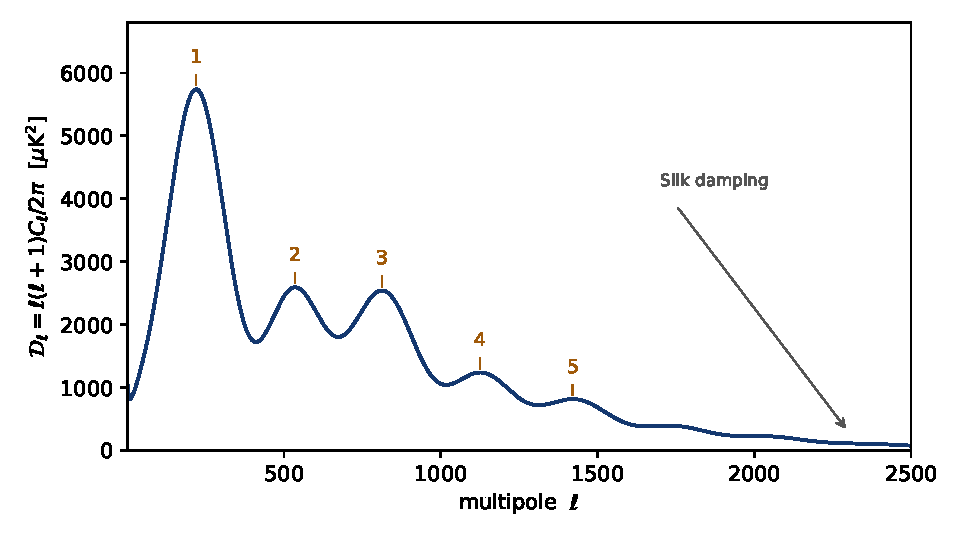
\includegraphics[width=0.49\textwidth]{figs/cmb_tt.pdf}\hfill
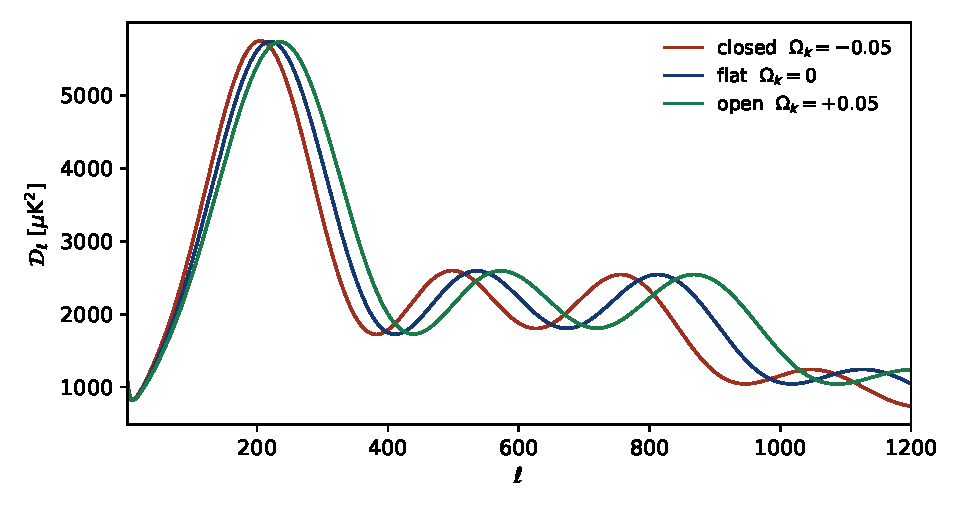
\includegraphics[width=0.49\textwidth]{figs/cmb_curvature.pdf}
\caption{\small שמאל: ספקטרום ה-\en{TT}, הפסגות האקוסטיות. ימין: הזזת הפסגה הראשונה עם העקמומיות.}
\end{figure}

\subsection{\en{BAO}: אותו סרגל בגלקסיות}
כל הפרעה התחילה כגל קול כדורי; בעידן הגרירה הגל "קפא" בבריונים במרחק $r_d$ מהמרכז, והחומר האפל נשאר במרכז. שניהם משכו זה את זה, ולכן בפונקציית המתאם של גלקסיות יש עודף במרחק נע $r_d\approx147\,\Mpc\approx100\,h^{-1}\Mpc$ (תנודות ב-$P(k)$).
\begin{equation}
\Delta\theta=\frac{r_d}{D_M(z)}\ \ (\text{רוחבי}),\qquad
\Delta z=\frac{r_d\,H(z)}{c}=\frac{r_d}{D_H(z)}\ \ (\text{לאורך קו הראייה}),\qquad
D_V=\big[z\,D_M^2D_H\big]^{1/3}.
\end{equation}
\begin{keybox}
\textbf{מה \en{BAO} מודד:} $D_M/r_d$ ו-$D_H/r_d$ כפונקציה של $z$. בלי ערך ל-$r_d$ מקבלים את $\Omega_m$ ואת $h\,r_d$ בלבד; עם $r_d$ מה-\en{CMB} או מ-\en{BBN} (עם $\Omega_bh^2$) מקבלים $H_0$. היחס $D_M/D_H$ (\en{Alcock--Paczynski}) לא תלוי ב-$r_d$ בכלל.
\end{keybox}

\begin{figure}[htbp]\centering
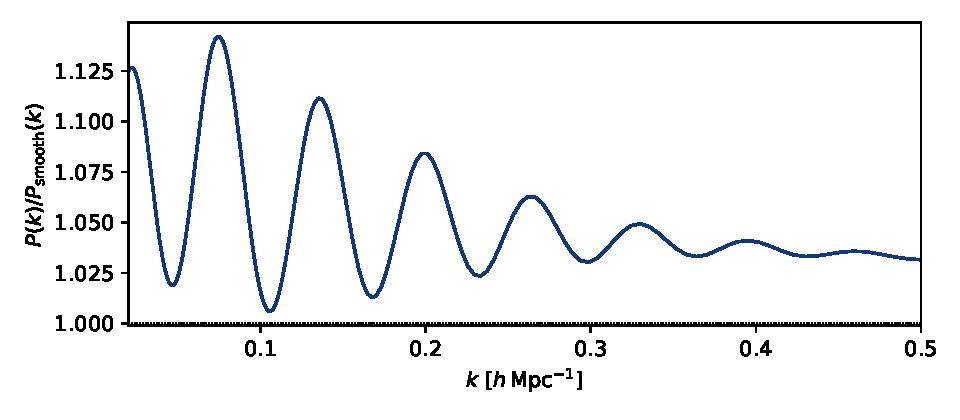
\includegraphics[width=0.55\textwidth]{figs/bao.pdf}
\caption{\small פיק ה-\en{BAO} בפונקציית המתאם, ב-$\approx100\,h^{-1}\Mpc$.}
\end{figure}

\subsection{\en{DESI DR2} והמתחים היום}
\en{DESI} (\en{Dark Energy Spectroscopic Instrument}; תוצאות \en{DR2} מתוך \en{arXiv:2503.14738}): $>14$ מיליון הסחות, שבע קבוצות עוקבים ב-$0.1<z<4.2$ (גלקסיות \en{BGS}, \en{LRG}, \en{ELG}, קוואזרים ויער \en{Ly$\alpha$}).
\begin{center}\small
\begin{tabular}{@{}p{5.6cm}p{1.4cm}p{8.8cm}@{}}
\toprule
צירוף נתונים & מודל & תוצאה \\ \midrule
\en{DESI} לבד & $\LCDM$ & $\Omega_m=0.2975\pm0.0086$, \ $h\,r_d=101.54\pm0.73\,\Mpc$ \\
\en{DESI+BBN} & $\LCDM$ & $H_0=68.51\pm0.58\,\kmsMpc$ \\
\en{DESI+CMB} & $w_0w_a$ & $w_0=-0.42\pm0.21$, $w_a=-1.75\pm0.58$; העדפה $3.1\sigma$ על $\Lambda$ \\
\en{DESI+CMB+SNe} & $w_0w_a$ & העדפה של \en{$2.8\sigma$ (Pantheon+), $3.8\sigma$ (Union3), $4.2\sigma$ (DESY5)} \\ \bottomrule
\end{tabular}
\end{center}

\begin{figure}[htbp]\centering
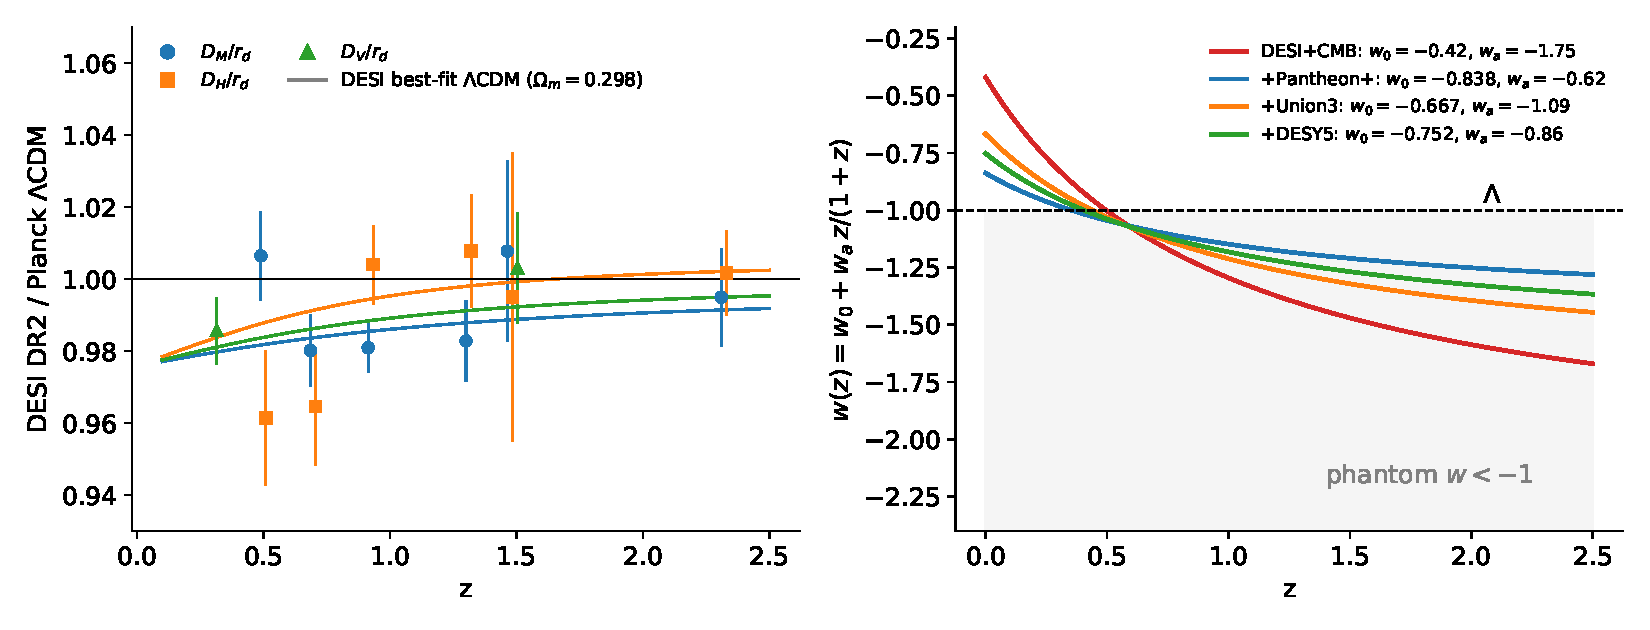
\includegraphics[width=\textwidth]{figs/fig_desi_bao.pdf}
\caption{\small שמאל: מרחקי \en{DESI DR2} ביחס ל-$\LCDM$ של \en{Planck}; הקו הרציף הוא ההתאמה הטובה ביותר של \en{DESI} ל-$\LCDM$ ($\Omega_m$ נמוך יותר). ימין: $w(z)$ של ארבע התאמות $w_0w_a$: כולן חוצות את $-1$ ליד $z\approx0.5$.}
\end{figure}

\textbf{שלושה מתחים, ומה לקחת מהם:}
\begin{enumerate}
\item \textbf{$H_0$.} סולם המרחקים (\en{SH0ES}, צפייניים${}+$\en{SNe}): $73.0\pm1.0$ (\en{Riess et al.\ 2022, ApJL 934, L7}). שיטות "הסרגל ההפוך" (\en{CMB}, או \en{BAO+BBN}): $67$--$68.5$. פער של $\sim4$--$5\sigma$. פתרון מוקדם חייב להקטין את $r_d$ בכ-$7\%$.
\item \textbf{$\Omega_m$.} \en{DESI} מעדיף $\Omega_m$ נמוך מעט מ-\en{Planck} ($0.315$); פער של $\sim2\sigma$ ב-$\LCDM$.
\item \textbf{אנרגיה אפלה דינמית.} $w_0>-1$, $w_a<0$: אנרגיה אפלה שהייתה "פנטום" ($w<-1$) בעבר ונחלשת היום. \emph{הסתייגויות:} תלוי בפרמטריזציה (\en{CPL}); תלוי בקטלוג הסופרנובות (טווח $2.8$--$4.2\sigma$); ומתקשר לגבול על מסת הנייטרינו ($\sum m_\nu<0.064\,\mathrm{eV}$ ב-$\LCDM$, לחץ לכיוון ערכים "שליליים").
\end{enumerate}
\textbf{קשר להרצאה 2:} אותה מכונה --- $\chi^2=\mathbf r^{\!\top}\mathsf C^{-1}\mathbf r$ בכל סל, עם מטריצה $2\times2$ ל-$(D_M/r_d,D_H/r_d)$. תרגיל הבית \en{HW 9B} בונה את כל הניתוח.

% ---------------------------------------------------------------------
\subsection*{תרגילים}
\begin{exercise}{מתי היקום נעשה שקוף?}
(א) הראו שמספר הפוטונים עם $E>13.6\,\mathrm{eV}$ לכל בריון הוא בערך $\eta^{-1}e^{-13.6\,\mathrm{eV}/k_BT}$ (עבור $k_BT\ll13.6\,\mathrm{eV}$, עד גורם פולינומי). (ב) עם $\eta=6\times10^{-10}$, מצאו את $T$ שבו המספר הזה הוא 1, ואת $z$ המתאים. (ג) \en{Saha} נותן $T\approx0.3\,\mathrm{eV}$. מה ההבדל בין רקומבינציה להתנתקות ($\Gamma_T=n_e\sigma_Tc=H$)?
\end{exercise}
\begin{solbox}
\textbf{פתרון.}\ (א) $n_\gamma(E>I)\propto\int_{I/T}^\infty x^2e^{-x}dx\approx(I/T)^2e^{-I/T}$; לבריון: $\eta^{-1}(I/T)^2e^{-I/T}$ עד קבוע $\sim0.4$.\\
(ב) $\eta^{-1}e^{-I/T}=1\Rightarrow T=I/\ln(1/\eta)=13.6/21.2=0.64\,\mathrm{eV}$, $z\approx2700$. הערכה גסה (הגורם הפולינומי מזיז את התשובה למטה).\\
(ג) רקומבינציה: $x_e$ יורד ל-$\sim0.5$ ב-$T\approx0.3\,\mathrm{eV}$ ($z\approx1300$). התנתקות: $n_e\sigma_Tc=H$, כש-$x_e\sim10^{-2}$, ב-$z\approx1090$. הפוטונים משתחררים מעט אחרי שהמימן נוצר.
\end{solbox}

\begin{exercise}{אופק הקול והפסגה הראשונה}
(א) בהזנחת $R$, ובחומר${}+$קרינה, הראו ש-
\[r_s=\frac{2c}{\sqrt3\,H_0\sqrt{\Omega_m}}\Big[\sqrt{a_\star+a_{\rm eq}}-\sqrt{a_{\rm eq}}\Big].\]
(ב) הציבו $\Omega_mh^2=0.143$, $z_\star=1090$, $z_{\rm eq}=3400$. כמה יוצא? מה יקרה כשמכניסים $R\approx0.6$? (התשובה המדויקת: $144\,\Mpc$.) (ג) עם $D_M(z_\star)=13.9\,\mathrm{Gpc}$, חשבו $\theta_\star$ ו-$\ell_A$. (ד) אם $\Omega_k=+0.05$, לאיזה כיוון זזה הפסגה?
\end{exercise}
\begin{solbox}
\textbf{פתרון.}\ (א) $r_s=\int c_s\,dt/a=\int c_s\,da/(a^2H)$ עם $a^2H=H_0\sqrt{\Omega_m}\sqrt{a+a_{\rm eq}}$; $\int_0^{a_\star}da/\sqrt{a+a_{\rm eq}}=2[\sqrt{a_\star+a_{\rm eq}}-\sqrt{a_{\rm eq}}]$.\\
(ב) $\frac{2c}{\sqrt3H_0\sqrt{\Omega_m}}=9150\,\Mpc$. בלי קרינה: $277\,\Mpc$; עם קרינה: $162\,\Mpc$; עם $R$ (מקטין את $c_s$ עד $\times0.79$ ב-$z_\star$): $144\,\Mpc$.\\
(ג) $\theta_\star=144/13\,900=0.0104$ רד' $=0.60^\circ$, $\ell_A=\pi/\theta_\star\approx302$ (הפסגה הראשונה ב-$\ell_1\approx220$ בגלל היסט פאזה).\\
(ד) $\Omega_k>0$ (סגור): $D_M$ קטן יותר, $\theta_\star$ גדול יותר, הפסגה זזה ל-$\ell$ נמוך יותר.
\end{solbox}

\begin{exercise}{נקודת \en{DESI} אחת}
\en{LRG2} ב-$z=0.706$: $D_M/r_d=17.35\pm0.18$, $D_H/r_d=19.46\pm0.33$. (א) עם $r_d=147.09\,\Mpc$, חשבו $D_M$ ו-$H(z)$. (ב) השוו ל-$\LCDM$ של \en{Planck} ($h=0.674$, $\Omega_m=0.315$). בכמה אחוזים ובכמה $\sigma$ שונה $H(0.706)$? (ג) חשבו את יחס \en{AP} $D_M/D_H$ בנתונים ובמודל. למה הוא לא תלוי ב-$r_d$ ו-$H_0$?
\end{exercise}
\begin{solbox}
\textbf{פתרון.}\ (א) $D_M=2552\,\Mpc$, $D_H=2862\,\Mpc$, $H=c/D_H=104.8\,\kmsMpc$.\\
(ב) \en{Planck}: $H(0.706)=67.36\sqrt{0.315(1.706)^3+0.685}=101.0$; $D_M=2604\,\Mpc$. \en{DESI}: $H$ גבוה ב-$3.7\%$ ($\sigma_H/H=1.7\%$, כלומר $2.2\sigma$); $D_M$ נמוך ב-$2.0\%$ ($\sim2\sigma$). זו הנקודה עם המשקל הגדול בהעדפה ל-$w_0w_a$.\\
(ג) $D_M/D_H=0.892$ (נתונים) מול $0.878$ (\en{Planck}). ביחס, $r_d$ ו-$c/H_0$ מתבטלים; נשאר רק $\int dz/E$ מול $1/E$, כלומר גיאומטריה טהורה.
\end{solbox}
